%==============================================================================
%  MATH 231 -- Linear Algebra I (Queens College, Fall 2026)
%  COMPUTATIONAL UNIT, PART 6 -- Gradient Descent
%
%  Section numbering runs CONTINUOUSLY across the parts of the computational
%  unit:
%
%      Part 1  MATH231_computational_1_operation_counting        Sections 1-4
%      Part 2  MATH231_computational_2_k_nearest_neighbours      Sections 5-10
%      Part 3  MATH231_computational_3_k_means_clustering        Sections 11-15
%      Part 4  MATH231_computational_4_gram_schmidt              Sections 16-20
%      Part 5  MATH231_computational_5_matrix_multiplication     Sections 21-23
%      Part 6  MATH231_computational_6_gradient_descent          Sections 24-27
%
%  Hence \setcounter{section}{23}: this part opens at Section 24.
%
%  STATUS: complete.  Sections 24-27.  The topic continues; Sec. 27.4 says so.
%
%  AUDIENCE: distributed to students.  No instructor-facing apparatus.
%
%  THIS PART DEPENDS ON THE VECTOR CALCULUS UNIT, Sec. 7.3 -- the gradient
%  points in the direction of steepest ascent.  That is the entire justification
%  for stepping along -f' / -grad f, and it is cited rather than re-argued.
%
%  THE STRUCTURAL MOVE OF THIS DOCUMENT, and the thing not to edit away:
%  Sec. 25.2 states the naive rule x_{k+1} = x_k - f'(x_k) and then RUNS IT on
%  f(x) = x^2, where it gives x_{k+1} = -x_k and oscillates 1, -1, 1, -1 forever,
%  never terminating.  The learning rate then arrives in Sec. 25.3 as the repair
%  for a failure the reader has already watched happen, rather than as an extra
%  knob introduced by decree.  f(x) = x^2 is chosen precisely because the whole
%  method is solvable in closed form on it: x_k = x_0 (1 - 2 eta)^k, so every
%  regime -- one-step, geometric, oscillating-convergent, oscillating-divergent
%  -- is visible analytically in Sec. 25.4 rather than asserted.
%
%  THE ITERATION CAP in the pseudocode is not boilerplate.  The eta = 1 case
%  above never satisfies the tolerance test, so without k_max the loop does not
%  return.  Sec. 26.1 says exactly that.
%
%  Sec. 26.2 keeps the honest caveat: a small derivative means a critical point,
%  not necessarily a minimum and certainly not a global one.  It points at
%  Sec. 14.1, where k-means already ran into local minima, so the reader meets
%  the idea as a recurrence rather than a new disappointment.
%
%  Compile with pdflatex (standard TeX Live packages only; uses tikz).
%==============================================================================
\documentclass[11pt]{article}

\usepackage[margin=1in]{geometry}
\usepackage{amsmath,amssymb,amsthm}
\usepackage[dvipsnames]{xcolor}
\usepackage{enumitem}
\usepackage{booktabs}
\usepackage{array}
\usepackage[hidelinks]{hyperref}
\usepackage{titlesec}
\usepackage{needspace}
\usepackage{tikz}
\usetikzlibrary{arrows.meta}

%------------------------------------------------------------------ style ----
\titleformat{\section}{\large\bfseries\sffamily}{\thesection.}{0.6em}{}
\titleformat{\subsection}{\normalsize\bfseries\sffamily}{\thesubsection.}{0.5em}{}
\titlespacing*{\section}{0pt}{14pt}{6pt}

\theoremstyle{plain}
\newtheorem{thm}{Theorem}[section]

\theoremstyle{definition}
\newtheorem{defn}{Definition}[section]
\newtheorem{ex}{Example}[section]
\theoremstyle{remark}
\newtheorem*{rmk}{Remark}
\newtheorem*{warn}{A common confusion}

\newcommand{\lookahead}{\par\smallskip\noindent
  \textbf{\sffamily\textcolor{RoyalBlue}{Looking ahead.}}\ \ignorespaces}
\newcommand{\lookback}{\par\smallskip\noindent
  \textbf{\sffamily\textcolor{ForestGreen}{From the vector calculus unit.}}\ \ignorespaces}

%--------------------------------------------------------------- notation ----
\newcommand{\R}{\mathbb{R}}
\newcommand{\vc}[1]{\mathbf{#1}}
\newcommand{\norm}[1]{\lVert #1\rVert}
\newcommand{\grad}{\nabla}
\newcommand{\lr}{\eta}

%--------------------------------------------------------------- pseudocode --
\newcommand{\kw}[1]{\textsf{\bfseries #1}}
\newcommand{\ind}{\hspace*{1.3em}}
\newcommand{\indd}{\hspace*{2.6em}}
\newcounter{algoline}
\newenvironment{algo}[2]{%
  \par\medskip\needspace{8\baselineskip}%
  \begin{center}\begin{minipage}{0.94\textwidth}%
  \hrule height 0.9pt \vspace{3pt}%
  \noindent{\sffamily\bfseries #1}\par\vspace{2pt}%
  \noindent{\small #2}\par\vspace{3pt}%
  \hrule height 0.4pt \vspace{5pt}%
  \begin{list}{\textbf{\arabic{algoline}:}}%
    {\usecounter{algoline}\setlength{\leftmargin}{2.3em}%
     \setlength{\labelwidth}{1.8em}\setlength{\labelsep}{0.5em}%
     \setlength{\itemsep}{2pt}\setlength{\topsep}{0pt}%
     \setlength{\parsep}{0pt}}%
}{%
  \end{list}\vspace{5pt}\hrule height 0.9pt%
  \end{minipage}\end{center}\medskip%
}

%------------------------------------------------------------- tikz helpers --
\tikzset{
  axisline/.style = {->, gray!75, thin},
  curveln/.style  = {RoyalBlue, very thick},
  steparr/.style  = {-{Stealth[length=2.2mm,width=1.7mm]}, BrickRed, thick}
}

\title{\vspace{-1.2cm}\textbf{\sffamily MATH 231 -- Linear Algebra I}\\[4pt]
       {\large\sffamily The Computational Unit, Part 6 \textbullet\
        Gradient Descent}\\[2pt]
       {\normalsize\sffamily Kiely Hall 326 \textbullet\
        Instructor: Kevin Bedoya}}
\author{}
\date{}

\begin{document}
\setcounter{section}{23}  % this part opens at Section 24; see the header note
\maketitle
\vspace{-1.6cm}

\noindent\textbf{About this document.} The vector calculus unit established that
the gradient points in the direction of steepest ascent, and remarked that an
algorithm follows from it. This is that algorithm. The whole of it is: to find a
low point, keep walking downhill.

\begin{center}
\renewcommand{\arraystretch}{1.2}
\begin{tabular}{@{}l l l@{}}
\toprule
\textbf{Part} & \textbf{Sections} & \textbf{Subject} \\
\midrule
1 & \S1--\S4    & operation counting, Big-O, floating point, error \\
2 & \S5--\S10   & $k$-nearest neighbours \\
3 & \S11--\S15  & $k$-means clustering \\
4 & \S16--\S20  & the Gram--Schmidt process \\
5 & \S21--\S23  & matrix multiplication as an algorithm \\
6 & \S24--\S27  & gradient descent \\
\bottomrule
\end{tabular}
\end{center}

\medskip
\noindent\textbf{Assumed.} From MATH~141: the derivative, and finding minima by
setting it to zero. From the vector calculus unit: the gradient (\S7.1) and,
above all, that $\grad f$ points in the direction of steepest ascent while
$-\grad f$ points in the direction of steepest descent (\S7.3). From this unit:
tolerances and floating-point comparison (\S4), and local minima as a failure
mode (\S14.1).

\medskip
\noindent\textbf{What you should be able to do afterwards.} Say when the
analytic method for finding a minimum stops being available; state the descent
step and explain why it moves against the derivative; explain what the learning
rate does and what goes wrong when it is too large or too small; write the
pseudocode with its stopping test and iteration cap; say what the algorithm does
and does not promise; and write the same algorithm in $n$ dimensions using the
gradient.

%==============================================================================
\section{The problem, and the obvious method}
%==============================================================================

%------------------------------------------------------------------------------
\subsection{A function to minimise}
%------------------------------------------------------------------------------
Start with the simplest interesting question in the subject: given a function
$f$, find the input at which it is smallest.

Take
\[
  f(x) = x^{2} .
\]
The answer is visible without any machinery. The graph is a parabola opening
upward, it is never negative, and it equals zero at $x=0$. So the minimum is at
$x^{\star}=0$ with value $f(x^{\star})=0$.

%------------------------------------------------------------------------------
\subsection{The analytic method}
%------------------------------------------------------------------------------
The method from MATH~141 confirms it. At a minimum the tangent line is flat, so
the derivative is zero there. Differentiate, set to zero, solve:
\[
  f'(x) = 2x,
  \qquad
  2x = 0,
  \qquad
  x^{\star} = 0 .
\]
Three steps, an exact answer, no approximation anywhere. When this works it is
unbeatable.

%------------------------------------------------------------------------------
\subsection{Where it stops working}
%------------------------------------------------------------------------------
Notice what the analytic method actually required: that the equation $f'(x)=0$
could be \emph{solved in closed form}. For $2x=0$ that is trivial. It is not
generally so.

Consider
\[
  f(x) = x^{6} - 3x^{4} + e^{x} + \tfrac{1}{1+x^{2}} .
\]
Differentiating is mechanical --- every rule needed is in the tables. But the
resulting equation $f'(x)=0$ mixes a polynomial with an exponential and a
rational function, and there is no algebraic procedure that isolates $x$. The
derivative exists, we can evaluate it at any point we like, and we still cannot
solve for the point where it vanishes.

This is the ordinary situation, not a contrived one. In the applications this
course is heading toward, $f$ may depend on thousands of variables and be
assembled from data rather than written as a formula. Setting a gradient to zero
and solving is out of the question.

So we need a method that never solves anything --- one that only ever
\emph{evaluates} $f$ and $f'$ at points of our choosing, and uses those numbers
to move somewhere better.

%==============================================================================
\section{Descending by steps}
%==============================================================================

%------------------------------------------------------------------------------
\subsection{The idea}
%------------------------------------------------------------------------------
Here is the whole plan. Start at a guess. Look at which way is downhill. Take a
step that way. Repeat until the ground is flat.

\lookback \S7.3 supplies the one fact this needs. At any point, $f$ increases
fastest in the direction of the gradient --- in one variable, the direction in
which the derivative points. To \emph{decrease} $f$ as fast as possible, move in
the opposite direction.

In one variable that reads: if $f'(x_k)>0$ then $f$ is rising to the right, so
step left; if $f'(x_k)<0$ then $f$ is rising to the left, so step right. Both
cases are captured by subtracting the derivative, since subtracting a positive
number moves left and subtracting a negative number moves right.

%------------------------------------------------------------------------------
\subsection{A first attempt}
%------------------------------------------------------------------------------
The simplest rule that does this is
\begin{equation}\label{eq:naive}
  x_{k+1} \;=\; x_k - f'(x_k) .
\end{equation}
Start somewhere, subtract the derivative, repeat, and stop when $|f'(x_k)|$ is
small enough that the ground is essentially flat.

Test it on $f(x)=x^{2}$, where $f'(x)=2x$. Starting from $x_0=1$:
\[
  x_{k+1} = x_k - 2x_k = -x_k .
\]
So the sequence is
\[
  1,\; -1,\; 1,\; -1,\; 1,\; \dots
\]
It jumps across the minimum to the mirror-image point, jumps back, and repeats
forever. It never gets closer to $x^{\star}=0$, and since $|f'(x_k)|=2$ at every
step, the stopping test never fires either. The loop does not terminate.

And this is the easiest possible function.

The direction was never the problem --- at $x=1$ the derivative is $+2$, and
moving left is correct. The problem is the \emph{distance}. The rule moved a
step of size $2$ when the minimum was only $1$ away, so it overshot, and it
overshoots by the same amount forever.

%------------------------------------------------------------------------------
\subsection{The learning rate}
%------------------------------------------------------------------------------
The fix is to stop taking the derivative at face value as a distance, and take
only a fraction of it. Introduce a positive number $\lr$ that scales the step:
\begin{equation}\label{eq:gd1}
  \boxed{\;x_{k+1} \;=\; x_k - \lr\,f'(x_k)\;}
\end{equation}

\begin{defn}[Learning rate]
The number $\lr>0$ in \eqref{eq:gd1} is the \textbf{learning rate}. It is a
\textbf{hyperparameter}: a value chosen by whoever runs the algorithm, not
computed by it, and not determined by $f$.
\end{defn}

\noindent The derivative still chooses the direction. The learning rate decides
how far to commit to it. Small $\lr$ means cautious steps; large $\lr$ means
aggressive ones.

%------------------------------------------------------------------------------
\subsection{Choosing it}
%------------------------------------------------------------------------------
On $f(x)=x^{2}$ we can see the entire effect of $\lr$ exactly, because the
iteration solves in closed form. With $f'(x)=2x$,
\[
  x_{k+1} = x_k - \lr(2x_k) = (1-2\lr)\,x_k
  \qquad\Longrightarrow\qquad
  x_k = (1-2\lr)^{k}\,x_0 .
\]
Every step multiplies the distance to the minimum by the fixed factor
$1-2\lr$. So the behaviour depends entirely on that one number:

\begin{center}
\renewcommand{\arraystretch}{1.45}
\begin{tabular}{@{}l l l@{}}
\toprule
\textbf{Learning rate} & \textbf{Factor $1-2\lr$} & \textbf{What happens} \\
\midrule
$\lr = 0.1$   & $0.8$   & shrinks steadily; converges \\
$\lr = 0.5$   & $0$     & lands exactly on $x^{\star}$ in one step \\
$\lr = 0.9$   & $-0.8$  & overshoots each time, but by less; still converges \\
$\lr = 1$     & $-1$    & overshoots exactly; oscillates forever \\
$\lr = 1.1$   & $-1.2$  & overshoots by more each time; diverges \\
\bottomrule
\end{tabular}
\end{center}

\noindent Convergence requires $|1-2\lr|<1$, that is $0<\lr<1$. The failure of
\eqref{eq:naive} was the row $\lr=1$ --- the naive rule was gradient descent with
the learning rate accidentally set to the one value that oscillates forever.

\begin{ex}[A run with $\lr=0.1$]
Starting from $x_0=1$, each step multiplies by $0.8$:
\begin{center}
\renewcommand{\arraystretch}{1.25}
\begin{tabular}{@{}c c c c@{}}
\toprule
$k$ & $x_k$ & $f(x_k)$ & $f'(x_k)$ \\
\midrule
$0$ & $1$        & $1$          & $2$ \\
$1$ & $0.8$      & $0.64$       & $1.6$ \\
$2$ & $0.64$     & $0.4096$     & $1.28$ \\
$3$ & $0.512$    & $0.262144$   & $1.024$ \\
$4$ & $0.4096$   & $0.167772$   & $0.8192$ \\
$5$ & $0.32768$  & $0.107374$   & $0.65536$ \\
\bottomrule
\end{tabular}
\end{center}
The iterates never reach $0$ exactly --- they approach it geometrically, which is
why a tolerance is needed rather than a test for equality. Reaching
$|f'(x_k)|<10^{-7}$ takes $76$ steps.
\end{ex}

\begin{center}
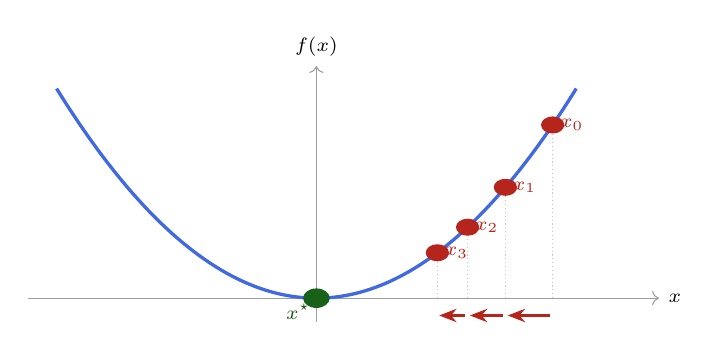
\begin{tikzpicture}[xscale=3.0,yscale=2.2]
  \draw[axisline] (-1.22,0) -- (1.45,0) node[right,font=\scriptsize,black]{$x$};
  \draw[axisline] (0,-0.14) -- (0,1.34) node[above,font=\scriptsize,black]{$f(x)$};
  \draw[curveln,domain=-1.10:1.10,smooth,samples=90] plot (\x,{\x*\x});
  % iterates: labels go to the RIGHT of each dot, into the space under the curve,
  % so they separate vertically instead of crowding horizontally
  \foreach \x/\lab in {1/{0}, 0.8/{1}, 0.64/{2}, 0.512/{3}}
    { \draw[gray!45,densely dotted] (\x,0) -- (\x,{\x*\x});
      \fill[BrickRed] (\x,{\x*\x}) circle (1.4pt);
      \node[right,font=\scriptsize,BrickRed,inner sep=2.5pt]
           at (\x,{\x*\x}) {$x_{\lab}$}; }
  % the leftward steps, along the axis
  \draw[steparr] (0.99,-0.10) -- (0.81,-0.10);
  \draw[steparr] (0.79,-0.10) -- (0.65,-0.10);
  \draw[steparr] (0.63,-0.10) -- (0.52,-0.10);
  \fill[ForestGreen!70!black] (0,0) circle (1.6pt);
  \node[below left,font=\scriptsize,ForestGreen!60!black,inner sep=2pt]
       at (0,0) {$x^{\star}$};
\end{tikzpicture}
\end{center}

\noindent Each step is smaller than the last, because the derivative --- which
sets the step size --- shrinks as the curve flattens. The algorithm slows down
automatically as it approaches the bottom.

\begin{warn}[Bigger is not faster]
It is tempting to read ``$\lr$ controls how fast we descend'' as ``larger $\lr$
means faster''. The table says otherwise: past $\lr=0.5$ the method starts
overshooting, and past $\lr=1$ it diverges outright, running away from the very
minimum it was asked to find. Too small is merely slow; too large is fatal.
\end{warn}

%------------------------------------------------------------------------------
\subsection{Why it is called a \emph{learning} rate}
%------------------------------------------------------------------------------
The name comes from machine learning, and the idea underneath it is simple.

A model is a rule with adjustable numbers inside it, called \textbf{weights}.
Feed it an input and it produces a guess. Compare that guess with the correct
answer and you get an error. Do this across all the available data and add the
errors up, and you have a single number measuring how wrong the model currently
is. That number is called the \textbf{loss}.

The loss depends on the weights --- change them and it changes. So the loss is a
function, the weights are its inputs, and \emph{making the model better means
making that function small}. Which is the problem this document is about.

Gradient descent does the adjusting. At each step it computes which way to nudge
the weights to reduce the error, and nudges them. Repeating that is what
``learning'' means here: a model learns by being shown that it was wrong and
correcting itself slightly in response.

The learning rate is the size of that correction. Set it small and the model
edges toward better weights slowly but steadily. Set it large and it lurches ---
possibly past the answer entirely, exactly as in the $\lr=1.1$ row above. Hence
the name: $\lr$ controls how fast the model learns, and whether it learns at all.

%==============================================================================
\section{The algorithm}
%==============================================================================

%------------------------------------------------------------------------------
\subsection{Pseudocode}
%------------------------------------------------------------------------------
\begin{algo}{Gradient descent (one variable)}{%
  \textbf{Input:} $f'$, a starting point $x_0$, a learning rate $\lr>0$, a
  tolerance $\tau>0$, an iteration cap $k_{\max}$.\quad
  \textbf{Output:} a point where $|f'|<\tau$, or a report of failure.}
\item $x \;\gets\; x_0$
\item \kw{for} $k = 0,1,2,\dots,k_{\max}$:
\item \ind $g \;\gets\; f'(x)$
        \hfill\textit{\small the slope where we are standing}
\item \ind \kw{if} $|g| < \tau$: \kw{return} $x$
        \hfill\textit{\small flat enough --- stop}
\item \ind $x \;\gets\; x - \lr\,g$
        \hfill\textit{\small step downhill}
\item \kw{return} failure --- $k_{\max}$ steps without reaching the tolerance
\end{algo}

\noindent Three of these lines deserve comment.

\textbf{Line 4 tests before stepping.} If the starting point already satisfies
the tolerance, the algorithm returns it immediately rather than taking a
pointless step first.

\textbf{The tolerance $\tau$ is a comparison against a small number, not against
zero.} As \S25.4 showed, the iterates approach the minimum without ever landing
on it, so a test for $f'(x)=0$ would never fire. Typical choices are
$\tau=10^{-7}$ for single precision or $\tau=10^{-14}$ for double, matching the
precisions of \S3.3 --- there is no point demanding an accuracy the arithmetic
cannot represent.

\textbf{The cap $k_{\max}$ is not boilerplate.} The $\lr=1$ row of \S25.4 runs
forever without ever satisfying the test on line 4. Without line 2's bound the
procedure would simply never return. A cap converts a hang into a reported
failure, which is the difference between a program you can debug and one you
have to kill.

%------------------------------------------------------------------------------
\subsection{What it does not promise}
%------------------------------------------------------------------------------
The algorithm returns a point where the derivative is small. It is worth being
precise about what that does and does not mean.

A small derivative marks a \emph{critical point} --- somewhere the graph is
locally flat. Minima are flat, but so are maxima and inflection points. In
practice descent will not settle on a maximum, since any step away from one
decreases $f$ and the method never comes back; but a flat stretch or a local dip
will hold it.

More importantly, ``a minimum'' is not ``the minimum''. If $f$ has several
valleys, the algorithm finds whichever one the starting point drains into. A
different $x_0$ can give a different answer, and nothing in the procedure can
tell you whether a lower valley exists somewhere it never looked.

This is the same limitation \S14.1 identified for $k$-means, and the same remedy
applies: run it several times from different starting points and keep the best
result. An algorithm that walks downhill can only report on the hill it was
dropped onto.

%==============================================================================
\section{In \texorpdfstring{$n$}{n} dimensions}
%==============================================================================

%------------------------------------------------------------------------------
\subsection{The generalisation}
%------------------------------------------------------------------------------
Nothing above was really about one variable. The argument was: move opposite to
the direction of steepest increase, by an amount controlled by $\lr$. In $\R^{n}$
that direction has a name --- it is $-\grad f$ --- and the rule transfers with no
change of idea at all.

\begin{defn}[Gradient descent]
Let $f:\R^{n}\to\R$. Given a starting point $\vc{x}_0\in\R^{n}$ and a learning
rate $\lr>0$, \textbf{gradient descent} generates the sequence
\begin{equation}\label{eq:gdn}
  \vc{x}_{k+1} \;=\; \vc{x}_k - \lr\,\grad f(\vc{x}_k) ,
\end{equation}
stopping when $\norm{\grad f(\vc{x}_k)} < \tau$.
\end{defn}

\noindent Set the two versions side by side:

\begin{center}
\renewcommand{\arraystretch}{1.6}
\begin{tabular}{@{}l l l@{}}
\toprule
 & \textbf{One variable} & \textbf{$n$ variables} \\
\midrule
The point        & $x_k\in\R$        & $\vc{x}_k\in\R^{n}$ \\
The direction    & $f'(x_k)$         & $\grad f(\vc{x}_k)$ \\
The step         & $x_k-\lr f'(x_k)$ & $\vc{x}_k-\lr\grad f(\vc{x}_k)$ \\
The stopping test& $|f'(x_k)|<\tau$  & $\norm{\grad f(\vc{x}_k)}<\tau$ \\
\bottomrule
\end{tabular}
\end{center}

\noindent Three substitutions and nothing else: the number becomes a vector, the
derivative becomes the gradient, and the absolute value becomes the norm. The
learning rate stays a single scalar --- one number scaling the whole vector step,
not one per coordinate.

The pseudocode of \S26.1 carries over verbatim under those substitutions.

%------------------------------------------------------------------------------
\subsection{An example}
%------------------------------------------------------------------------------
\begin{ex}
Minimise $f(x,y)=x^{2}+y^{2}$, whose minimum is plainly at the origin. From the
vector calculus unit, $\grad f(x,y)=[\,2x,\,2y\,]$, so \eqref{eq:gdn} reads
\[
  \vc{x}_{k+1}
  = \vc{x}_k - \lr\,[\,2x_k,\,2y_k\,]
  = (1-2\lr)\,\vc{x}_k .
\]
This is the one-variable result again, now applied to both coordinates at once:
the whole vector shrinks by the factor $1-2\lr$ every step. Starting from
$\vc{x}_0=[\,1,\,2\,]$ with $\lr=0.1$,
\[
  [\,1,\,2\,] \to [\,0.8,\,1.6\,] \to [\,0.64,\,1.28\,]
  \to [\,0.512,\,1.024\,] \to \cdots
\]
converging to $[\,0,\,0\,]$ along the straight line through the origin.
\end{ex}

%------------------------------------------------------------------------------
\subsection{One learning rate, many directions}
%------------------------------------------------------------------------------
The example above was unusually kind: the function curves at the same rate in
both directions, so a single $\lr$ suits both equally.

Change it to
\[
  f(x,y) = x^{2} + 10y^{2} ,
\]
a bowl far steeper along $y$ than along $x$, and the two coordinates now want
different treatment. The gradient is $[\,2x,\,20y\,]$, so a step multiplies the
$x$-part by $1-2\lr$ and the $y$-part by $1-20\lr$. Convergence needs
\emph{both} factors below $1$ in size, which forces $\lr<0.1$ --- a restriction
imposed entirely by the steep direction. The shallow $x$ direction is then
crawling, multiplied by at least $0.8$ each step, purely because a larger $\lr$
would make $y$ diverge.

The single scalar $\lr$ must serve every direction at once, and the worst
direction sets the limit.

\lookahead That tension is the starting point for most of what follows.
Everything that improves on plain gradient descent is, in one way or another, an
attempt to stop the steepest direction from dictating the step size for all the
others --- by adapting $\lr$ as the run proceeds, by giving each coordinate its
own effective rate, or by using curvature information to rescale the step. The
quantity that measures how badly a problem suffers from this also has a name,
and it is one this unit has met before in a different guise.

We will continue.

\end{document}
